% !TEX root = Projektarbeit.tex

\chapter{Das Kernelmodul - Der hardwarespezifische Treiber} %TODO ?
Nachdem nun die Grundfunktionen eines Linux Kernelmoduls vorgestellt wurden, sollen im Folgenden die spezifischen Funktionen für die Kommunikation mit dem Waveshare e-Paper Display über die \texttt{UART}-Schnittstelle erläutert werden.

Der hardwarespezifische Treiber für das e-Paper-Display ist kein von Grunde auf neu geschriebener Treiber, sondern wird als sogenannter \glqq Stacked~Driver\grqq~gestapelt auf schon vorhandenen Low-Level-Treibern des Linux-Kernels aufgebaut. 
Um die \texttt{UART}-Kommunikation im Kernel zu ermöglichen, nutzt Treiber auf dem \texttt{serial-core} Low-Level-Treiber für serielle Kommunikation. 

\section{Zuordnung zwischen Display und Treiber} %TODO \citep{elinuxDevTree} \citep{lwnDevTree} 
Eine der größeren Änderungen im Linux Kernel war die Einführung des Device Trees für Computer, die auf ARM Prozessoren basieren. Damit werden fest in den Kernel einkompilierte Board Beschreibungsdateien langsam ersetzt. Nun werden Informationen über verfügbare Schnittstellen, wie beispielsweise UART- oder I2C-Interfaces, dynamisch zum Kernel dazu geladen, der so auch auf der ARM-Plattform generischer verwendbar sein soll. 

Dies führt dazu, dass auch im Kernelmodul eine flexiblere Art der Zuordnung zwischen Hardware und Treiber genutzt werden muss und über sogenannte \glqq Compatible-Strings\grqq~(Listing \ref{lst:compatible-strings}, Zeile 4 bzw. 16/17) realisiert wird. Die Compatible-Strings sind in Device Tree Description Files (Ausschnitt siehe Listing \ref{lst:compatible-strings}) für beispielsweise einen Bus oder einen Port definiert. 

Im Treiber wird eine Zuordnung zu dem hier benötigten \texttt{UART}-Interface statt. Es wird definiert, dass der Waveshare Treiber geladen werden soll, wenn ein Gerät an einer Schnittstelle des Prozessors, die die Compatible-Strings \texttt{ti,am3352-uart} oder \texttt{ti,omap3-uart} trägt und die \texttt{UART}-Interfaces des Beaglebone Blacks bezeichnet, erkannt wird. Die Definition auf welche Compatible-Strings geachtet werden soll, geschieht in der \mintinline{c}{struct of_device_id waveshare_uart_of_ids[]} (Listing \ref{lst:compatible-strings}, Zeile 15).

In der Struktur \texttt{platform\_driver}, die die Adressen der hardwarespezifischen Treiberfunktionen enthält, wird die \mintinline{c}{struct of_device_id waveshare_uart_of_ids[]} für den Waveshare-Treiber verwaltet (Listing \ref{lst:compatible-strings}, Zeile 29).


\begin{listing} [H]
\caption{Verknüpfung von Hardware und Treiber über Compatible-Strings}
\label{lst:compatible-strings}
\begin{minted} [frame=lines, framesep=2mm, fontsize=\footnotesize, linenos] {c}
// In den Kernelquellen
// linux/arch/arm/boot/dts/am33xx.dtsi
uart0: serial@44e09000 {
			compatible = "ti,am3352-uart", "ti,omap3-uart";
			ti,hwmods = "uart1";
			clock-frequency = <48000000>;
			reg = <0x44e09000 0x2000>;
			interrupts = <72>;
			status = "disabled";
			dmas = <&edma 26>, <&edma 27>;
			dma-names = "tx", "rx";
		};

// Im Waveshare Treiber waveshare.c
static const struct of_device_id waveshare_uart_of_ids[] = {
	{ .compatible = "ti,omap3-uart" ,},
	{ .compatible = "ti,am3352-uartti" ,},
	{ },
};
MODULE_DEVICE_TABLE(of, waveshare_uart_of_ids);

static struct platform_driver waveshare_serial_driver = {
	.probe = waveshare_uart_probe,
	.remove = waveshare_uart_remove,
	.id_table = waveshare_uart_of_ids,
	.driver = {
		.name = "waveshare_uart",
		.owner = THIS_MODULE,
		.of_match_table = waveshare_uart_of_ids,
	},
};
\end{minted}
\end{listing}


\subsection{Hotplugging} %TODO \citep{hotplug}
Eine besondere Bedeutung bei der Zuordnung zwischen Hardware und Treiber hat das Macro \mintinline{c}{MODULE_DEVICE_TABLE()} (Listing \ref{lst:compatible-strings}, Zeile 20). Es hilft bei der Realisierung des Hotplugging Mechanismus im Kernel, also für ein neu erkanntes Gerät automatisch den passenden Treiber zu laden. Das Macro wird dafür zu Variablen aufgelöst, die Informationen über die angegebene Struktur mit den Compatible-Strings enthalten. Wird das kompilierte Modul zum Kernel geladen und mit \texttt{depmod} dessen Abhängigkeiten aufgelöst, sucht \texttt{depmod} auch nach den von dem Macro erzeugten Variablen und generiert aus diesen für jeden Bustyp Map-Files, z.B. \texttt{modules.usbmap} für Geräte am USB-Bus. Wird ein neues Gerät erkannt, werden die Map-Dateien auf die erzeugten Variablen durchsucht und falls vorhanden, der zugehörige Treiber geladen. \\

Das folgende Bild \ref{pic:hotplugging} zeigt die Logs des Kernels nachdem das Kernelmodul in das richtige Verzeichnis kopiert, der Befehl \texttt{depmod -a} ausgeführt wurde und das \texttt{UART1}-Interface des Beaglebone Black mit \texttt{echo BB-UART1 > /sys/devices/platform/bone\_capemgr/slots} aktiviert wurde. Es zeigt ab [246.157316] die Aktivierung von \texttt{UART1} und anschließend ab [246.236404] die Log- und Debugmeldungen der Initialisierung des Waveshare-Treibers, ohne dass dieser explizit von Hand geladen worden wäre.


\begin{figure}[H]
  \centering
  \fbox{
   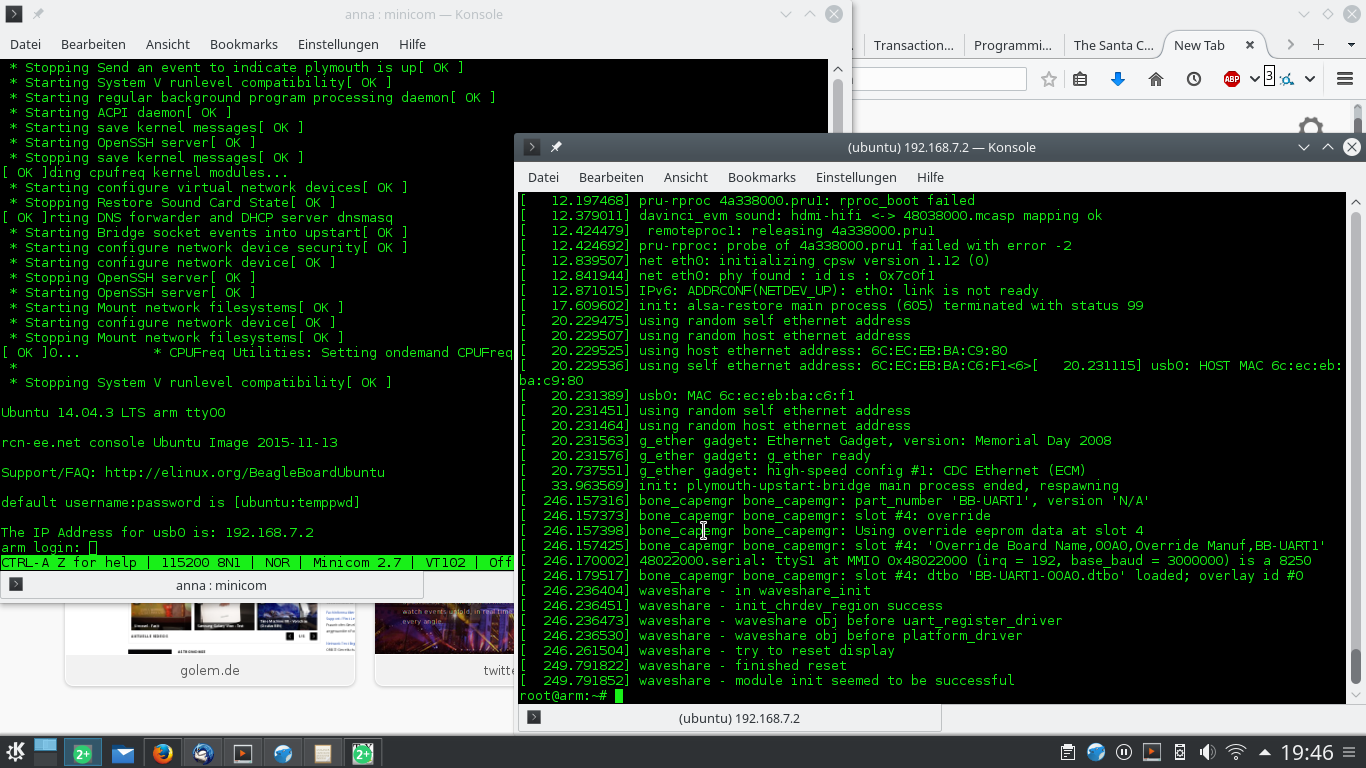
\includegraphics[scale=0.65]{dmesg_treiber_geladen}
  }
  \caption{Kernellog Hotplugging}
  \label{pic:hotplugging}
\end{figure}


\section{Die serielle Kommunikation über das \texttt{UART}-Interface im Kernel} %TODO titel ändern \citep{platformLWN} 
Im folgenden wird die Hardwareinitialisierung im Kernel über das \texttt{UART}-Interface vorgestellt. Über dieses Hardware-Interface soll eine serielle Kommunikation realisiert werden. Dazu wird der Serial Core Treiber des Kernels genutzt, auf dem der Waveshare-Treiber als \glqq Stacked Driver\grqq~aufgebaut wird. Serielle Geräte, wie auch das Waveshare-Display, fallen in Linux unter die Kategorie der \texttt{tty}-Geräte. Benannt nach der ältesten seriellen Schnittstelle blieb dieser Name bis heute erhalten. \\ %TODO hier evtl /proc/tty/waveshare ... o.ä. erwähnen 

\subsection{Registrierung beim Serial Core Treiber} %TODO Titel ändern
Die Initialisierung des \texttt{UART}-Treibers beginnt schon in der Modul-Initialisierung. 
Hier wird mit der Funktion \mintinline{c}{uart_register_driver()} (Listing \ref{lst:hwabhInit}, Zeile 21) der Waveshare Treiber beim Serial Core Treiber des Kernels registriert. Dazu wird der Funktion die Struktur \mintinline{c}{struct uart_driver waveshare_uart_driver} (Zeile 1) übergeben. Darin sind Besitzer, Namen sowie die maximale Anzahl an unterstützten \texttt{UART} Ports und eine eventuell angebotene Konsole angegeben. 

Darauf wird mit der Funktion \mintinline{c}{platform_driver_register()} wird der Treiber beim Kernel noch als Plattform Treiber angemeldet. In der hier übergebenen Struktur \\ 
\mintinline{c}{struct platform_driver waveshare_serial_driver} (Listing \ref{lst:hwabhInit}, Zeile 9) sind die Funktionen hinterlegt, die für die weitergehende Initialisierung der seriellen Kommunikation zur Hardware genutzt werden. 
Unabhängig vom verwendeten Hardwaretyp werden diese als \texttt{probe} und \texttt{release} bezeichnet. Der Nutzen der Struktur \texttt{waveshare\_uart\_of\_ids} wurde schon zuvor im Kapitel über Hotplugging erläutert. \\

Nach einer erfolgreichen Initialisierungen sind neue Einträge im \texttt{proc}- und im \texttt{sys}-Dateisystem sichtbar. Dabei handelt es sich z.B. um \texttt{/proc/tty/driver/waveshare} sowie um \texttt{/sys/bus/platform/drivers/waveshare\_uart}, die durch die vorgestellten Funktionen angelegt werden. 


\begin{listing} [H]
\caption{Hardwareabhängige Initialisierung in \texttt{waveshare\_init}}
\label{lst:hwabhInit}
\begin{minted} [frame=lines, framesep=2mm, fontsize=\footnotesize, linenos] {c}
static struct uart_driver waveshare_uart_driver = {
	.owner = THIS_MODULE,
	.driver_name = "waveshare",
	.dev_name = DEVICENAME,
	.nr =  1,
	.cons = NULL,
};

static struct platform_driver waveshare_serial_driver = {
	.probe = waveshare_uart_probe,
	.remove = waveshare_uart_remove,
	.id_table = waveshare_uart_of_ids,
	.driver = {
		.name = "waveshare_uart",
		.owner = THIS_MODULE,
		.of_match_table = waveshare_uart_of_ids,
	},
};


static int __init waveshare_init (void) {
[...]
        if (uart_register_driver(&waveshare_uart_driver)) {
		goto free_uart;
	}

	if (platform_driver_register(&waveshare_serial_driver)) {
		goto free_platform;
	}
[...]   
}
\end{minted}
\end{listing} 

\subsection{Probleme}
Nach dieser Modulinitialisierung sollte normalerweise automatisch die in der Struktur \mintinline{c}{struct platform_driver waveshare_serial_driver} angegebene \texttt{probe()}-Funktion aufgerufen werden. Leider passiert dies nicht und die weitere hardwarespezifische Initialisierung in dieser Funktion bleibt unberührt. Woran genau dies scheitert ist sehr schwer herauszufinden, da Debugging im Kernel wie schon erwähnt, nur in einem begrenzten Rahmen möglich ist.

Sowohl \mintinline{c}{uart_register_driver()} als auch \mintinline{c}{platform_driver_register()} laufen nicht in die Fehlerbehandlung. Es kann also davon ausgegangen werden, dass beide Funktionen korrekt ausgeführt wurden und der Treiber im Kernel bzw. beim Serial Core Treiber registriert wurde. Auch die Einträge im \texttt{proc}- und \texttt{sys}-Dateisystem, \\ 
\texttt{/proc/tty/driver/waveshare} sowie \texttt{/sys/bus/platform/drivers/waveshare\_uart}, die bei einem korrekten Ablauf erwartet werden, sind vorhanden. Ebenfalls für eine korrekte Ausführung an dieser Stelle spricht, dass bei einem expliziten Aufruf der \texttt{probe()}-Funktion eine Fehlermeldung erscheint, die besagt, dass der Plattform Treiber schon registriert wurde. Die \texttt{probe()}-Funktion wird dabei nicht betreten. \\ %TODO nochmal genau nachsehen, was könnte hier noch alles aufgeführt werden 

Nach längerer, erfolgloser Fehlersuche wurde in Absprache mit dem betreuenden Professor an dieser Stelle abgebrochen. Dennoch existieren die prototypischen Funktionen \texttt{probe()} und \texttt{release()} zur hardwarespezifischen Initialisierung bzw. Abmeldung, sowie Funktionen, die darstellen wie ohne die vorhandenen Schwierigkeiten die tatsächliche Kommunikation zum Waveshare Display, anhand der zur Verfügung stehenden API sowie Referenzimplementierungen aus dem Linux Kernel, realisiert werden sollte. Durch besagte Schwierigkeiten konnten diese nicht auf ihre Korrektheit überprüft werden, dennoch sollen diese Funktionen im weiteren Verlauf dieser Arbeit vorgestellt werden, um zu zeigen was der Treiber im geplanten Funktionsumfang leisten sollte.


\subsection{Die probe()-Funktion} %TODO titel ändern
Während in der \texttt{init}-Funktion vor allem das Kernel Modul selbst initialisiert wird, übernimmt die \texttt{probe}-Funktion die Initialisierung des Gerätes, dass am \texttt{UART}-Interface erkannt wurde. Diese Trennung ist nötig, um die Hotplugging Funktionalität zu realisieren. Die folgende Implementierung basiert auf den zur Verfügung stehenden APIs und Referenz-Implementierungen im Linux-Kernel. Die Funktionsfähigkeit konnte nicht überprüft werden. \\

Die \texttt{probe}-Funktion (Listing \ref{lst:hwabhProbe}, Zeile 9) beginnt Speicher für die Struktur \\ 
\texttt{waveshare\_uart\_port} zu mit \texttt{devm\_kzalloc()} zu allozieren. Besonders an dieser Methode ist, dass der von der Struktur belegte Speicher an die Existenz des Treibers geknüpft ist und danach automatisch freigegeben wird. 
Der hier in dieser Struktur gespeicherte Port, an dem das Gerät angeschlossen ist, wird als Referenz in der Struktur \texttt{uart\_port} des Serial Core Treibers gespeichert. Anschließend werden Ressourcen für das Plattform-Gerät reserviert und unter \texttt{port->membase} wird über die Funktion \texttt{devm\_ioremap\_resource()} (Listing \ref{lst:hwabhProbe}, Zeile 24) der I/O-Speicher dieses Geräts zugreifbar gemacht. Über diesen Speicher sollen Daten zwischen Treiber und Hardware übertragen werden. 
In \texttt{port->ops} (Zeile 32) wird eine Referenz auf Funktionen gespeichert, die das Verhalten des über das \texttt{UART}-Interface angeschlossenen Geräts definieren. Im weiteren wird vorgestellt, wie eine solche Funktion für die Initialisierung des e-Paper-Displays aussehen könnte.
Im letzten interessanten Part der \texttt{probe}-Funktion wird mit der Funktion \texttt{uart\_add\_one\_port()} (Zeile 36) der vorher definierte \texttt{UART}-Port mit der \texttt{uart\_driver}-Struktur beim Serial Core Treiber registriert. 
Abschließend werden \texttt{platform\_set\_drvdata()} die treiberspezifischen Daten für das Plattformgerät gesetzt. \\

Das Gegenstück zur \texttt{probe()}-Funktion ist die \texttt{release()}-Funktion, hier \\ 
\texttt{waveshare\_uart\_remove()}, in der die getätigten Registrierungen beim Serial Core Treiber bzw. beim Kernel aufgehoben werden müssen. Allozierter Speicher muss nicht explizit freigegeben werden, da dies durch die besondere Allokation automatisch geschieht. So bleibt nur noch mit der Funktion \texttt{uart\_remove\_one\_port()} die Registrierung beim Serial Core Treiber zu lösen. 

\begin{listing} [H]
\caption{Hardwareabhängige Initialisierung in \texttt{waveshare\_uart\_probe()}}
\label{lst:hwabhProbe}
\begin{minted} [frame=lines, framesep=2mm, fontsize=\footnotesize, linenos] {c}
struct waveshare_uart_port {
	struct uart_port port;
};

static struct uart_ops waveshare_uart_ops = {
	.startup = waveshare_uart_startup,
};

static int waveshare_uart_probe (struct platform_device *pdev) {
	
	struct waveshare_uart_port *wav_port;
	struct uart_port *port;
	struct resource *mem_res;
	unsigned int baud;
	
	wav_port = devm_kzalloc (&pdev->dev, sizeof (struct waveshare_uart_port), GFP_KERNEL);
	if (!wav_port) {
		return -EINVAL;
	}

	port = &wav_port->port;
	
	mem_res = platform_get_resource (pdev, IORESOURCE_MEM, 0);
	port->membase = devm_ioremap_resource(&pdev->dev, mem_res);
	if (IS_ERR(port->membase)) {
		return PTR_ERR(port->membase);
	}

	port->mapbase = mem_res->start;
	port->dev = &pdev->dev;

	port->ops = &waveshare_uart_ops;

	baud = 115200;

	if (uart_add_one_port(&waveshare_uart_driver, &wav_port->port)) {
		goto free_uart_add_one_port;
	}
	
	platform_set_drvdata(pdev, wav_port);
	
	return 0;

free_uart_add_one_port:
	return -1;	
}
\end{minted}
\end{listing} 

\subsection{Prototypische Steuerung des e-Paper Displays}
Wie schon angerissen, soll erläutert werden wie die Funktion zum Start des Displays, auf die in der Struktur \mintinline{c}{struct uart_ops waveshare_uart_ops} unter \texttt{.startup} verwiesen wird, realisiert werden könnte. 
Da das e-Paper Display in der Lage ist die Darstellung auch ohne Spannungszufuhr zu halten soll beim Start zuerst eine Leerung des Displayinhalts durchgeführt werden, um mit einem definierten Ausgangszustand, also einer leeren Anzeige, zu starten. Laut dem Manual des Herstellers (Literaturverzeichnis \cite{waveshareMan}), lautet der benötigte Befehlsrahmen \texttt{A5 00 09 2E CC 33 C3 3C 82}. 

Um diesen übermitteln zu können wird eine Hilfsfunktion \mintinline{c}{waveshare_uart_write()} (Listing \ref{lst:displayReset}, Zeile 1) definiert, die ein einzelnes Byte über schon erwähntem I/O-Speicher überträgt. 

Die Funktion \mintinline{c}{waveshare_uart_startup()} selbst, stellt daher nur noch die Übertragung des Befehlsrahmens über die Hilfsfunktion dar. \\

Auf diese Weise könnten weitere Befehle sowie das Setzen von Text und Grafiken entsprechend der vorgesehenen Befehlsrahmen realisiert werden, um die Funktionalität des Treibers zu vervollständigen. Text zur Darstellung auf dem Display könnte über die \texttt{write()}-Funktion oder Attributdateien im \texttt{sysfs} in den Kernelspace eingelesen werden, dort verarbeitet und in den entsprechenden Befehlsrahmen eingebettet an das Display gesendet werden.

\begin{listing} [H]
\caption{Reset des Displays}
\label{lst:displayReset}
\begin{minted} [frame=lines, framesep=2mm, fontsize=\footnotesize, linenos] {c}
static inline void waveshare_uart_write (struct waveshare_uart_port *up, 
  int offset, char value) {
	return writeb (value, up->port.membase + offset);
}

static int waveshare_uart_startup (struct uart_port *port) {

	struct waveshare_uart_port *wave_port = 
	  container_of (port, struct waveshare_uart_port, port);
	
	waveshare_uart_write (wave_port, 0x00, 0xA5);
	waveshare_uart_write (wave_port, 0x00, 0x00);
	waveshare_uart_write (wave_port, 0x00, 0x09);
	waveshare_uart_write (wave_port, 0x00, 0x2E);
	waveshare_uart_write (wave_port, 0x00, 0xCC);
	waveshare_uart_write (wave_port, 0x00, 0x33);
	waveshare_uart_write (wave_port, 0x00, 0xC3);
	waveshare_uart_write (wave_port, 0x00, 0x3C);
        waveshare_uart_write (wave_port, 0x00, 0x82);
		
	return 0;
}
\end{minted}
\end{listing}

%TODO weiter mit den nicht mehr ausgeführten funktionen

% X %TODO geraeteinitialisierung usw..


%TODO was wäre wenn es geklappt hätte... fehlt evt doch nur ein struct? unterschlag ich jetzt...

\chapter{Fazit}